\documentclass[
	% -- opções da classe memoir --
	12pt,				% tamanho da fonte
	openright,			% capítulos começam em pág ímpar (insere página vazia caso preciso)
	oneside,			% para impressão em frente e verso. Oposto a oneside
	a4paper,			% tamanho do papel.
	% -- opções da classe abntex2 --
	chapter=TITLE,		% títulos de capítulos convertidos em letras maiúsculas
	%section=TITLE,		% títulos de seções convertidos em letras maiúsculas
	%subsection=TITLE,	% títulos de subseções convertidos em letras maiúsculas
	%subsubsection=TITLE,% títulos de subsubseções convertidos em letras maiúsculas
	% -- opções do pacote babel --
	english,			% idioma adicional para hifenização
	french,				% idioma adicional para hifenização
	spanish,			% idioma adicional para hifenização
	brazil				% o último idioma é o principal do documento
	]{abntex2}

% ---
% Pacotes básicos 
% ---
\usepackage{lmodern}			% Usa a fonte Latin Modern
\usepackage{mathptmx}			% Usa a fonte Times New Roman
\usepackage[T1]{fontenc}		% Selecao de codigos de fonte.
\usepackage[utf8]{inputenc}		% Codificacao do documento (conversão automática dos acentos)
\usepackage{lastpage}			% Usado pela Ficha catalográfica
\usepackage{indentfirst}		% Indenta o primeiro parágrafo de cada seção.
\usepackage{color}				% Controle das cores
\usepackage{graphicx}			% Inclusão de gráficos
\usepackage{subcaption}				% Inclusão de gráficos lado a lado
\usepackage{microtype} 			% para melhorias de justificação
\usepackage{tabularx,ragged2e}	% Para inserir tabelas
\usepackage{multirow}			% Para mesclar células
\usepackage[dvipsnames,table,xcdraw]{xcolor}		% Permite adicionar cores nas linhas de tabelas
\usepackage{fancyvrb}			% Permite adicionar arquivos de texto
\usepackage[portuguese, ruled, linesnumbered]{algorithm2e} % Uso de algoritmos
\usepackage{amsfonts}			% Permite usar notação de conjuntos
\usepackage{amsmath}			% Permite citar equações
\usepackage{amsthm}				% Permite criar teoremas e experimentos
\usepackage{amssymb}            % Usei para o símbolo de transposto
\usepackage[font={bf, small}, labelsep=endash, labelfont=bf]{caption}	% Faz legenda de figuras ficarem em negrito
\usepackage[final]{pdfpages}
\usepackage{textcomp}           % para não dar erro no gensymb
\usepackage{gensymb}            % Para inserir o símbolo de grau em ângulos
\usepackage{enumitem}           % Para criar listas "numeradas" por letras (no abntex2 tem alineas no lugar)
\usepackage{bm,amsbsy}          % Para usar símbolos em negrito

\newcolumntype{L}{>{\RaggedRight\arraybackslash}X}
% ---

\usepackage[alf, abnt-emphasize=bf]{abntex2cite}	% Citações padrão ABNT
\usepackage{modelo-ufpa/ufpa}

% Muda o título de lista de ilustrações para lista de figuras
\addto\captionsbrazil{%
  \renewcommand{\listfigurename}%
    {Lista de Ilustrações}%
	\renewcommand{\listtablename}%
    {Lista de Tabelas}%
}

% Permite utilizar figuras sem precisar colocar o caminho absoluto
\graphicspath{{imagens/}}

% Define o ambiente de experimentos
\theoremstyle{definition}
\newtheorem{experimento}{Experimento}[section]
\newcommand{\experimentoautorefname}{Experimento}

%% Novo estilo
\makepagestyle{estilo_pretextual} %%% escolha um nome
  \makeevenhead{estilo_pretextual}{}{}{\ABNTEXfontereduzida \textbf \thepage}
  \makeoddhead{estilo_pretextual}{}{}{\ABNTEXfontereduzida \textbf \thepage}

%% Customiza comando \pretextual
\renewcommand{\pretextual}{
  \pagenumbering{roman} %%% ou \pagenumbering{Roman}
  \aliaspagestyle{chapter}{estilo_pretextual}% customizing chapter pagestyle
  \pagestyle{estilo_pretextual}
  \aliaspagestyle{cleared}{empty}
  \aliaspagestyle{part}{estilo_pretextual}
}

% ---
% Ajusta a marca \textual para que a numeração volte a ser arábica
% nos elementos textuais
\let\oldtextual\textual        % copia o comando \textual anterior para \oldtextual
\renewcommand{\textual}{%
  \oldtextual%
  \pagenumbering{arabic} % volta à numeração arábica
}
% ---


% ---
% Informações de dados para CAPA, FOLHA DE ROSTO e FICHA CATALOGRÁFICA
% ---
\universidade{Universidade Federal do Pará}
\instituto{Instituto de Tecnologia}
\faculdade{Programa de Pós-Graduação em Engenharia Elétrica}
\titulo{Nome do trabalho}
\autor{Weverson Vieira do Nascimento}
\local{Belém - PA}
\data{\the\year}
\tipotrabalho{Dissertação}
\grau{Mestre em Engenharia Elétrica } % manter o espaço no final
\preambulo{Dissertação apresentada como exigência parcial para obtenção do grau de \imprimirgrau pela \imprimiruniversidade. Área de concentração: Engenharias.}
\sobrenome{Nascimento}
\nome{Weverson Vieira do}
\palavraschave{
primeira.
segunda.
terceira.
quarta.
quinta.
}

% orientadores
\orientador{Prof. Dr. Fulano}
%\coorientador{Prof. Dr. Ciclano}
\datadadefesa{Data da Defesa: \underline{\qquad \qquad\qquad}}% janeiro de 2018}
\conceito{Conceito: \underline{\qquad\qquad\qquad}}
\primeiromembrodabanca{Prof.ª Dra. Ciclana}
\segundomembrodabanca{Prof. Dr. Fulano}
%\terceiromembrodabanca{Prof. Dr. Nome Sobrenome}
%\quartomembrodabanca{Prof. Dr. Outro Nome}
\faculdadecoordenador{Prof.ª Dra. Maria Emília de Lima Tostes}
% ---
% informações do PDF
\makeatletter
\hypersetup{
     	%pagebackref=true,
		pdftitle={\imprimirtitulo}, 
		pdfauthor={\imprimirautor},
    	pdfsubject={\imprimirpreambulo},
	    pdfcreator={LaTeX with abnTeX2},
		pdfkeywords={\imprimirpalavraschave}, 
		colorlinks=true,       		% false: boxed links; true: colored links
    	linkcolor=black,          	% color of internal links
    	citecolor=black,        		% color of links to bibliography
    	filecolor=magenta,      		% color of file links
		urlcolor=black,
		bookmarksdepth=4,
        breaklinks=true
}
\makeatother
% --- 

% --- 
% Espaçamentos entre linhas e parágrafos 
% --- 

% O tamanho do parágrafo é dado por:
\setlength{\parindent}{1.3cm}

% Controle do espaçamento entre um parágrafo e outro:
\setlength{\parskip}{0.2cm}  % tente também \onelineskip
\linespread{1.5} % espaçamento entre linhas

% ---
% compila o indice
% ---
\makeindex
% ---


% ----
% Início do documento
% ----
\begin{document}
\selectlanguage{brazil}
\frenchspacing 

% ----------------------------------------------------------
% ELEMENTOS PRÉ-TEXTUAIS
% ----------------------------------------------------------
% \pretextual

% ---
% Capa (obrigatório)
% ---
\imprimircapa
% ---

% ---
% Folha de rosto (obrigatório)
% ---
\imprimirfolhaderosto
% ---
% a ficha catalográfica oficial é a gerada pela biblioteca da instituição
% deve constar na versão final
% na ausência, usar a gerada pelo modelo
% \begin{fichacatalografica}
%     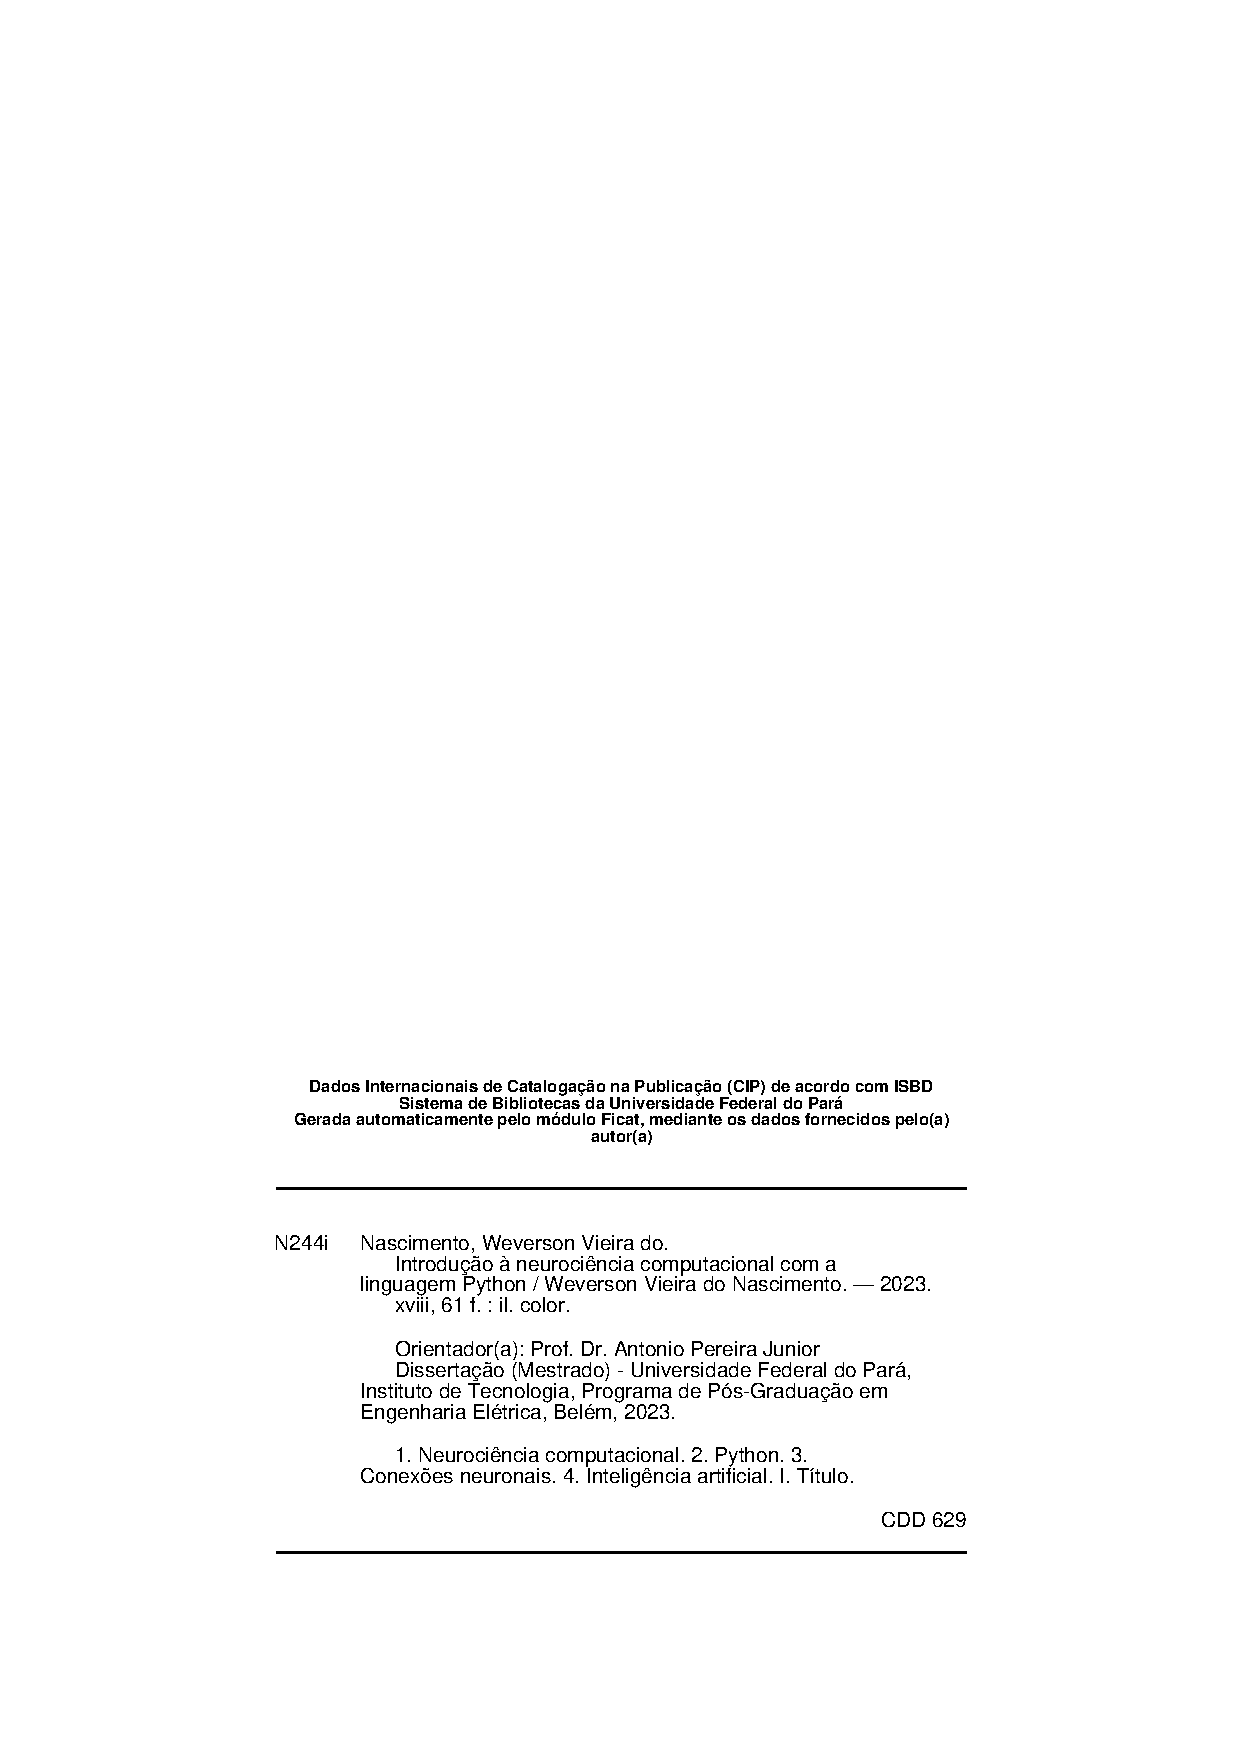
\includepdf{modelo-ufpa/ficha.pdf}
% \end{fichacatalografica}
\newpage
\begin{fichacatalografica}
	\imprimirfichacatalografica
\end{fichacatalografica}

% ---
% Inserir folha de aprovação (obrigatório)
% ---
% na versão final deve-se incluir a folha assinada
% \includepdf{folhadeaprovacao_final.pdf}
\begin{folhadeaprovacao}
	\ufpaPaginaDeAprovacao
    %\imprimirfolhadeaprovacao
\end{folhadeaprovacao}
% ---

% ---
% Dedicatória (opcional)
% ---
\begin{dedicatoria}
   \vspace*{\fill}
   \noindent
   \begin{flushright}
      \textit{escreva}\\
      \textit{aqui}\\
      \textit{a}\\
      \textit{dedicatória}
   \end{flushright}
\end{dedicatoria}
% ---

% ---
% Agradecimentos (opcional)
% ---
\begin{agradecimentos}
a escrever.
\end{agradecimentos}
% ---

% ---
% Epígrafe (opcional - NBR 10520)
% ---
\begin{epigrafe}
    \vspace*{\fill}
	\begin{flushright}
		\textit{``texto da epígrafe''\\
		autor}
	\end{flushright}
\end{epigrafe}
% ---

% ---
% RESUMOS
% ---
\setlength{\absparsep}{18pt}
\begin{resumo}
%O  resumo  deve  ressaltar  o  objetivo,  o  método,  os  resultados  e  as  conclusões  do  documento.  A  ordem  e  a  extensão destes itens dependem do tipo de resumo (informativo ou indicativo) e do tratamento que cada item recebe no documento original.
%O  resumo  deve  ser  composto  de  uma  sequência  de  frases  concisas,  afirmativas  e  não  de  enumeração  de  tópicos. Recomenda-se o uso de parágrafo único.
%A  primeira  frase  deve  ser  significativa,  explicando  o  tema  principal  do  documento.  A  seguir,  deve-se  indicar  a informação sobre a categoria do tratamento (memória, estudo de caso, análise da situação etc.).
texto do resumo

\textbf{Palavras-chave}: \imprimirpalavraschave
\end{resumo}

\begin{resumo}[Abstract]
 \begin{otherlanguage*}{english}
abstract

   \vspace{\onelineskip}
 
   \noindent 
   \textbf{Keywords}: escrever manualmente.
 \end{otherlanguage*}
\end{resumo}

% ---
% inserir lista de ilustrações (opcional)
% ---
\pdfbookmark[0]{\listfigurename}{lof}
\listoffigures*
\cleardoublepage
% ---

% ---
% inserir lista de quadros (não existe na norma, consta como ilustração)
% ---
%\pdfbookmark[0]{\listofquadrosname}{loq}
%\listofquadros*
%\cleardoublepage
% ---

% ---
% inserir lista de tabelas (opcional)
% ---
\pdfbookmark[0]{\listtablename}{lot}
\listoftables*
\cleardoublepage
% ---

% ---
% inserir lista de algoritmos (não consta na norma)
% ---
%\pdfbookmark[0]{\listalgorithmcfname}{loa}
%\imprimirlistadealgoritmos
%\cleardoublepage
% ---

% ---
% inserir lista de abreviaturas e siglas (opcional)
% ---
% listar em ordem alfabética
\begin{siglas}
\item[UFPA] Universidade Federal do Pará
\end{siglas}
% ---

% ---
% inserir lista de símbolos (opcional)
% ---
% inserir na ordem que aparecem no texto
\begin{simbolos}
\item[$\alpha$] Estrela de maior brilho de uma constelação % eu gosto de ver estrelas (literalmente)
\end{simbolos}
% ---

% ---
% inserir o sumario (obrigatório - NBR 6027)
% ---
\pdfbookmark[0]{\contentsname}{toc}
\tableofcontents*
\cleardoublepage
% ---



% ----------------------------------------------------------
% ELEMENTOS TEXTUAIS
% ----------------------------------------------------------
\textual

% ---
% algumas pessoas gostam de escrever os capítulos em .tex separados
% se for o caso eles devem ser incluídos no texto principal usando o comando abaixo.
% colocar tantos "includes" quantos forem os capítulos do texto.
% um inconveniente disso é não aparecer a estrutura de tópicos completa (pelo menos no overleaf);
% é possível colocando os \chapter no main, e manter o restante nos .tex separados,
% mas as seções ainda ficariam separadas, e o include, por padrão, gera uma nova página, o que
% pode ser complicado de lidar
% ---
\chapter{Introdução}\label{cap:introducao}
\section{Contexto}

\section{Justificativa}

\section{Objetivos}
\subsection{Objetivo Geral}
Elaborar um roteiro para execução de um curso introdutório em neurociências computacionais usando linguagens de programação livres

\subsection{Objetivos Específicos}
\begin{itemize}
\item Obter uma bibliografia robusta para servir de base na elaboração do roteiro
\item Criar um conjunto de códigos contendo exemplos dos conceitos apresentados ao longo do roteiro
\item Consolidar o material criado em uma estrutura de fácil uso por interessados no tema em questão
\end{itemize}

\section{Metodologia}

\section{Estrutura do Trabalho}
O trabalho está estruturado da seguinte maneira: o Capítulo~\ref{cap:teoria} mostra os elementos da base teórica apresentada. Uma breve apresentação de definições sobre fisiologia, equações diferenciais ordinárias, probabilidade, noções sobre algoritmos e linguagem de programação são mostradas. O Capítulo~\ref{cap:temas} contém os temas teóricos e práticos que constituem o roteiro em si. O Capítulo~\ref{cap:conclusoes} contém as conclusões acerca do trabalho e os desdobramentos possíveis para este.

\chapter{Base teórica}\label{cap:teoria}
\section{Introdução}\label{sec:teoria_intro}
Dada a variedade de estudantes que podem ingressar em um curso de neurociência computacional, muitos deles podem não ter tido algumas disciplinas de base que são necessárias para um bom entendimento do conteúdo apresentado. Por isso, este capítulo contém uma base teórica útil para um nivelamento dos estudantes das mais diversas áreas. As sessões seguintes contemplam conteúdos de neurobiologia, equações diferenciais ordinárias, probabilidade e algoritmos.

\section{Neurobiologia básica}\label{sec:fisiologia}
O neurônio é a unidade básica do sistema nervoso. É composto pelo corpo celular (chamado de soma), dendritos, que recebem sinais de outros neurônios, axônio, que transmite os sinais a serem recebidos por outros neurônios, e terminais axônicos, que são as extremidades do axônio e se conectam com os dendritos de outros neurônios. Como outras células do corpo humano, o neurônio é composto por íons e moléculas, ambas podendo possuir cargas positivas ou negativas. A célula neuronal é revestida por uma bi-camada lipídica, e geralmente o interior dela possui uma maior concentração de cargas negativas, fazendo com que o potencial de membrana ($V_m$), que é a diferença de potencial entre a parte interna e a externa da célula neuronal ($V_M=V_{dentro}-V_{fora}$), fique a maior parte do tempo com valor negativo. O potencial de membrana se altera quando há o fluxo de íons através dos poros de canais iônicos (Figura~\ref{fig:membrananeuronio}).

\begin{figure}[tb]
	\centering
	\caption[Membrana do neurônio]{Membrana do neurônio}
	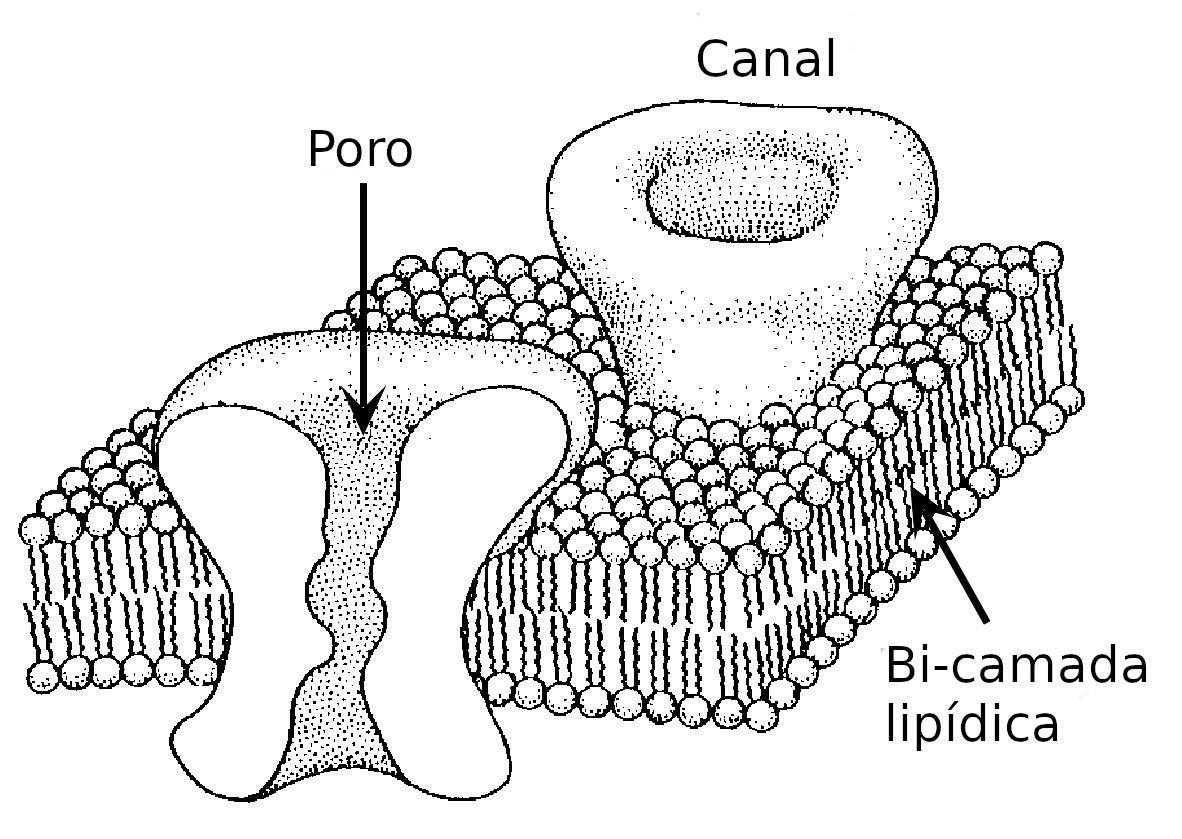
\includegraphics[width=0.55\linewidth]{figs/membrana_neuronio}
	\label{fig:membrananeuronio}
	\\
	Fonte: adaptado de \cite{hille_ionic_1992}
	%% adaptado de hille 1992 (pág. 170 pdf)
\end{figure}

Os canais iônicos são canais proteicos na membrana da célula neuronal e permitem a movimentação de íons através deles, como mostrado na Figura~\ref{fig:canaisions}. Podem ser de dois tipos: com ou sem portão. Canais sem portão estão sempre abertos, enquanto os com portão podem abrir ou fechar, dependendo do valor do potencial de membrana, e por isso são chamados de canais iônicos dependentes de tensão. Quando o fluxo de corrente elétrica de todos os íons é equilibrado dentro e fora da célula neuronal (ou seja, o potencial de membrana não se altera), ele é chamado de potencial de repouso (ou de equilíbrio). O valor típico é próximo de $-70\ mV$. O valor do potencial de repouso é calculado com base na concentração de cada íon dentro e fora da célula neuronal usando a equação de Nernst, dada por:
$$
E_A=\frac{k_BT}{z_Aq_e}ln\Big(\frac{A_{fora}}{A_{dentro}}\Big)
$$
sendo $A$ o íon, $z_A$ a carga do íon, $A_{fora}$ e $A_{dentro}$ a concentração desse íon fora e dentro da célula neuronal, respectivamente, $T$ a temperatura absoluta (em Kelvin), $k_B$ a a constante de \textit{Boltzmann} ($1,39*10^{-23}\ JK^{-1}$) e $q_e$ a carga elétrica fundamental ($1,6*10^{-19}\ C$). Os valores de cargas, concentração e potencial de Nernst para alguns íons são apresentados na Tabela~\ref{tab:concentracao_nernst}.

\begin{figure}[tb!]
	\centering
	\caption[Canais iônicos de potássio]{Canais iônicos de potássio. Em \textbf{a} os íons de potássio saem da célula, causando um excesso de cargas positivas fora e negativas dentro. Em \textbf{b} o fluxo para fora e dentro é igual, causando equilíbrio}
	\label{fig:canaisions}
	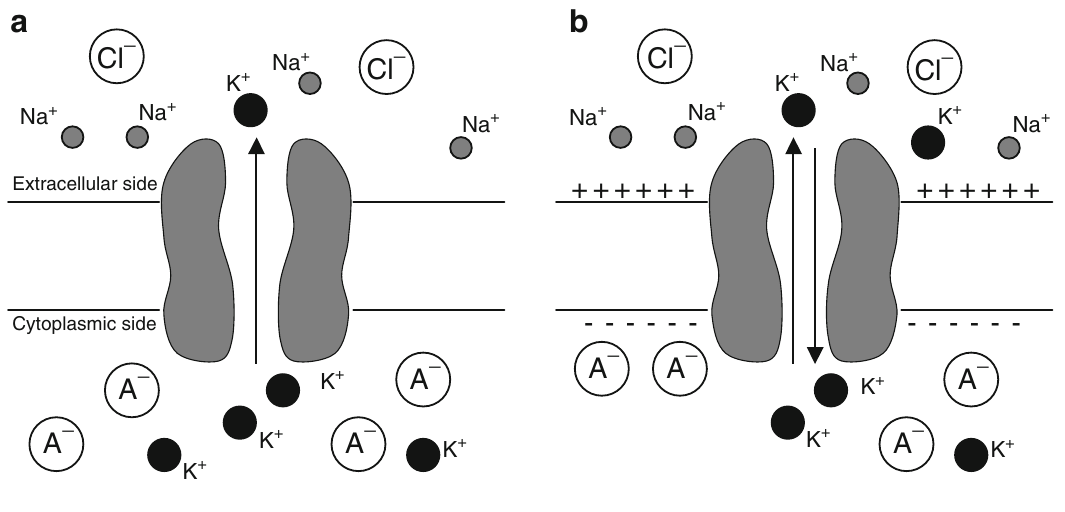
\includegraphics[width=0.7\linewidth]{figs/canais_ions}
	\\
	\cite{ermentrout_mathematical_2010}
\end{figure}

\begin{table}
	\centering
	\caption[Concentração de íons]{Concentração de íons}
	\label{tab:concentracao_nernst}
	\begin{tabular}{c|c|c|c|c}
		\hline
		Íon & Carga & Conc. interna ($nM$) & Conc. externa ($nM$) & Potencial de reversão ($mV$) \\
		\hline
		Sódio & +1 & 15 & 120 & 61,6 \\
		\hline
		Potássio & +1 & 150 & 6 & -86,1 \\
		\hline
		Cloreto & -1 & 52 & 560 & -65 \\
		\hline
		Cálcio & +2 & 50 & 2 & 141,7 \\
		\hline
	\end{tabular}
\end{table}

Fora do repouso, a diferença de potencial entre o interior e o exterior do neurônio produz movimentação iônica. Quando íons positivos (como $Na^+$ ou $Ca^{2+})$ entram na célula neuronal, o potencial de membrana fica menos positivo (até próximo de 0 mV), fenômeno conhecido como despolarização. De maneira semelhante, quando íons negativos (como $K^+$) saem da célula neuronal, ou negativos (como $Cl^-$) entram, o potencial de membrana fica mais negativo, fenômeno conhecido como hiperpolarização. Devido ao excesso de cargas negativas no interior da célula neuronal, e a existência de cargas positivas no exterior, a membrana do neurônio acaba funcionando como um capacitor, criando uma capacitância ($C_m$). O fluxo de íons através de canais sem portão é considerado constante, podendo ser agrupado em um elemento chamado de vazamento (\textit{leak}, em inglês), possuindo um potencial ($E_l$) e uma condutância ($G_l$), que é a facilidade desse elemento permitir o fluxo de corrente (o inverso da resistência). Com isso, é possível escrever uma equação relacionando o potencial de membrana da célula neuronal e os elementos de vazamento, como segue:
$$
\frac{\mathrm{d}V_m}{\mathrm{d}t}=G_l(E_l-V_m)/C_m
$$
que é dada na forma de uma equação diferencial, detalhada na seção seguinte.

\section{Equações diferenciais ordinárias}\label{sec:eqdif}
\begin{itemize}
	\item Equação diferencial ordinária: uma equação relacionando uma função desconhecida $y(t)$, algumas derivadas de $y(t)$ e a variável $t$, geralmente representando o tempo \cite{adkins_ordinary_2012}
	\item Ordem: a ordem da maior derivada que aparece na equação diferencial
	\item $t$: variável independente
	\item $y$: variável dependente (depende de $t$)
	\item A solução é uma família de equações, que depende da escolha de constantes
\end{itemize}

\begin{figure}[htb!]
	\centering
	\caption{Soluções $y(t) = t + 1 + ce^t$ da equação $y'=y-t$ para vários $c$}
	\label{fig:solucao}
	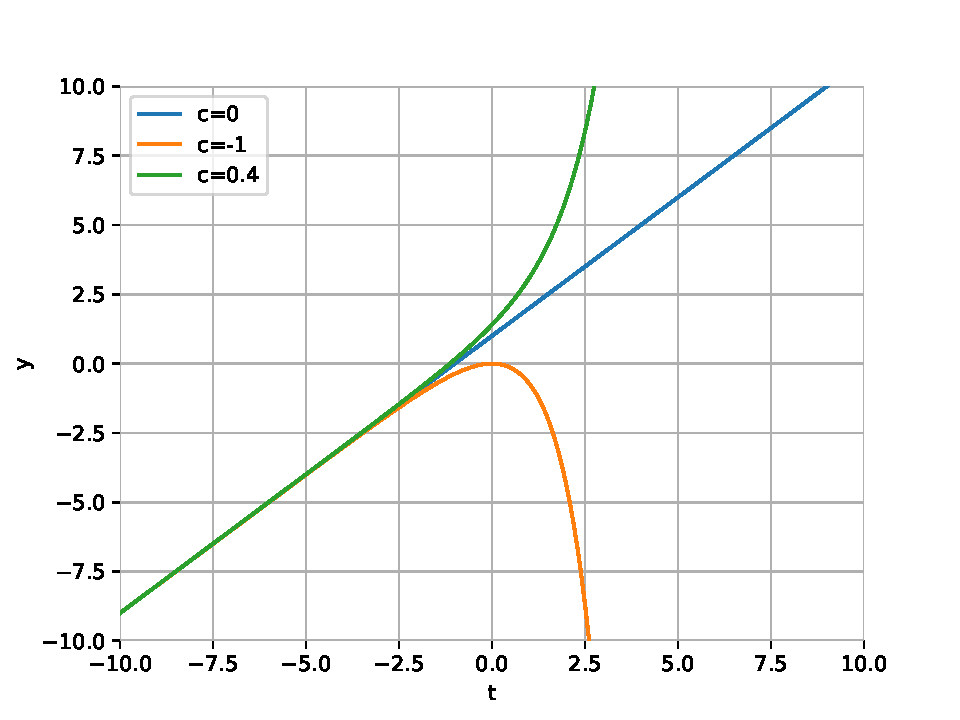
\includegraphics[width=0.7\linewidth]{figs/solucao}
\end{figure}


\subsection{Exemplos}
\subsubsection{Decaimento radioativo}
Segundo a lei do decaimento radioativo, a taxa na qual os átomos radioativos desintegram é proporcional ao número total de átomos radioativos presente. Sendo $N(t)$ o número de átomos radioativos no tempo $t$, então $N'(t)$ é a taxa de mudança. A lei do decaimento radioativo é a que segue:

$$N'(t) = -\lambda N(t)$$
onde $\lambda$ é a constante de decaimento.

\begin{figure}[htb!]
	\centering
	\caption{Decaimento radioativo ($\lambda = 0,5$)}
	\label{fig:decaimento}
	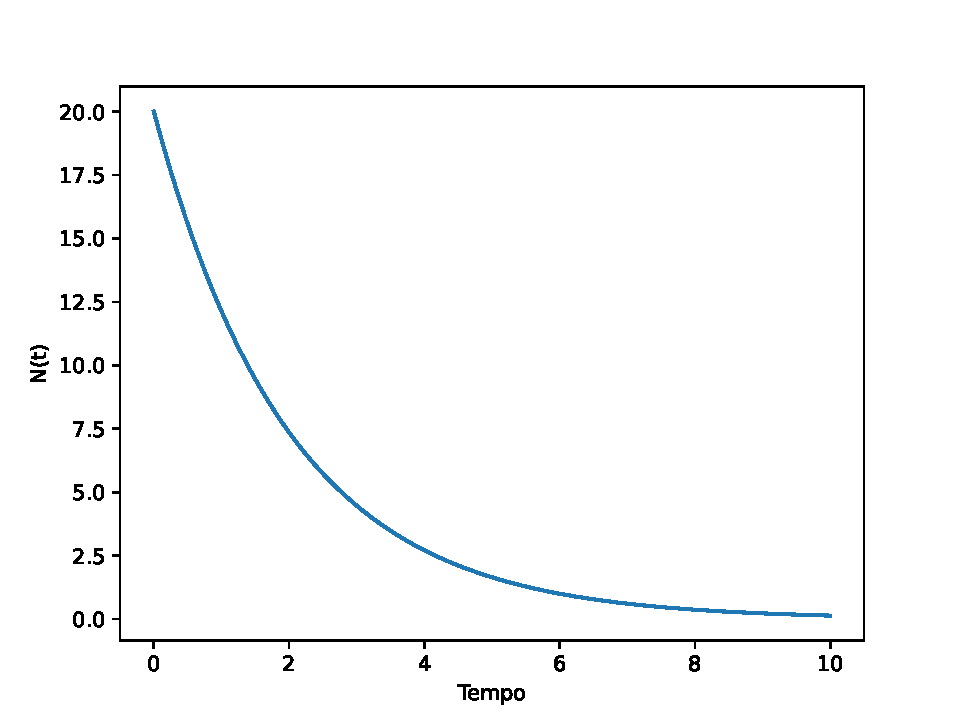
\includegraphics[width=0.7\linewidth]{figs/decaimento}
\end{figure}

\subsubsection{Equações de Lotka-volterra}
Também conhecidas como equações predador-presa, são um par de equações diferenciais de primeira ordem, frequentemente usadas para descrever a dinâmica de sistemas biológicos de interação entre duas espécies, uma como predadora e a outra como presa. As populações de cada uma das espécies são dadas pelo par de equações:

$$
x' = ax - bxy
$$$$
y' = dxy - cy
$$
onde:\\
$
x: \text{população da presa}\\
y: \text{população do predador}\\
x', y': \text{taxas de variação de cada população}\\
a, b, c, d: \text{parâmetros que descrevem a interação entre as espécies}
$

\begin{figure}[htb!]
	\centering
	\caption{Sistema de Lotka-Volterra ($a$ = 1,5; $b$ = 1; $c$ = 3; $d$ = 1)}
	\label{fig:lotka-volterra}
	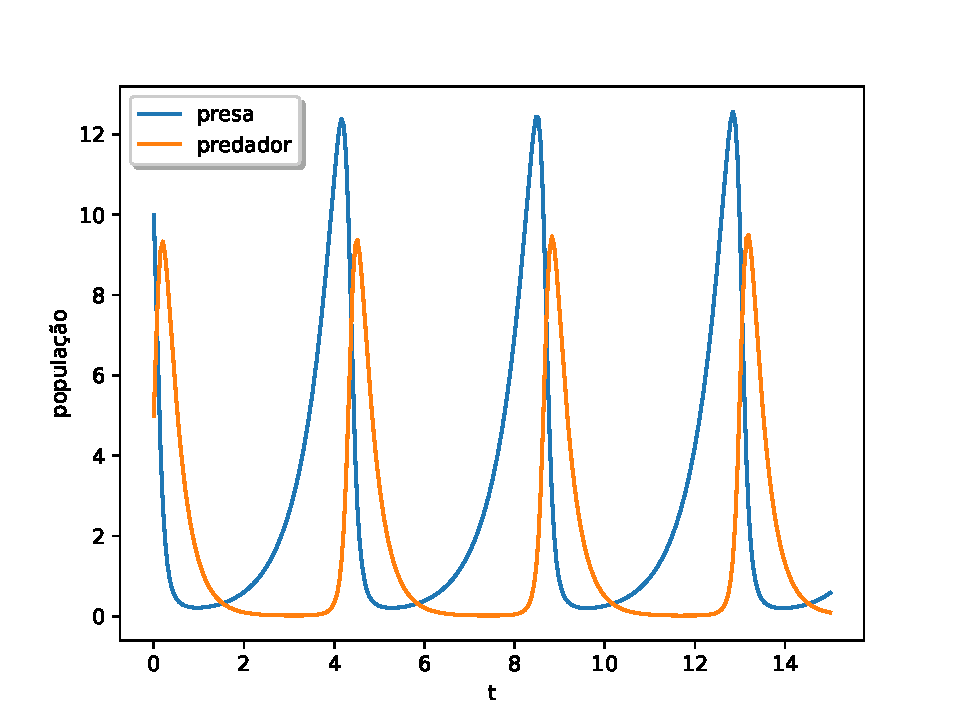
\includegraphics[width=0.7\linewidth]{figs/lotka-volterra}
\end{figure}


\subsubsection{Trajetória pendular}
O pêndulo é um dispositivo que contém uma massa atrelada a um fio e que oscila em torno de um ponto fixo. A equação do movimento para o ângulo $\theta$ (o ângulo que o pêndulo faz com a vertical) é:

$$
\frac{d^2\theta}{dt^2} = -\frac{1}{Q}\frac{d\theta}{dt} + \sin{\theta} + d\cos{\Omega t}
$$
onde:\\
$
t: \text{tempo}\\
Q: \text{fator de qualidade}\\
d: \text{amplitude}\\
\Omega: \text{frequência}
$
\\\\
Como se trata de uma equação diferencial de segunda ordem, é necessária a redução para duas equações de primeira ordem. Fazendo a substituição de variáveis $\omega = \frac{d\theta}{dt}$ podemos reescrever da seguinte maneira:

$$
\frac{d\theta}{dt} = \omega
$$$$
\frac{d\omega}{dt} = -\frac{1}{Q}\omega + \sin{\theta} + d\cos{\Omega t}
$$

\begin{figure}[htb!]
	\centering
	\caption[Trajetória pendular]{Trajetória pendular ($Q$ = 2; $d$ = 1,5; $\Omega$ = 0,65)}
	\label{fig:pendulo}
	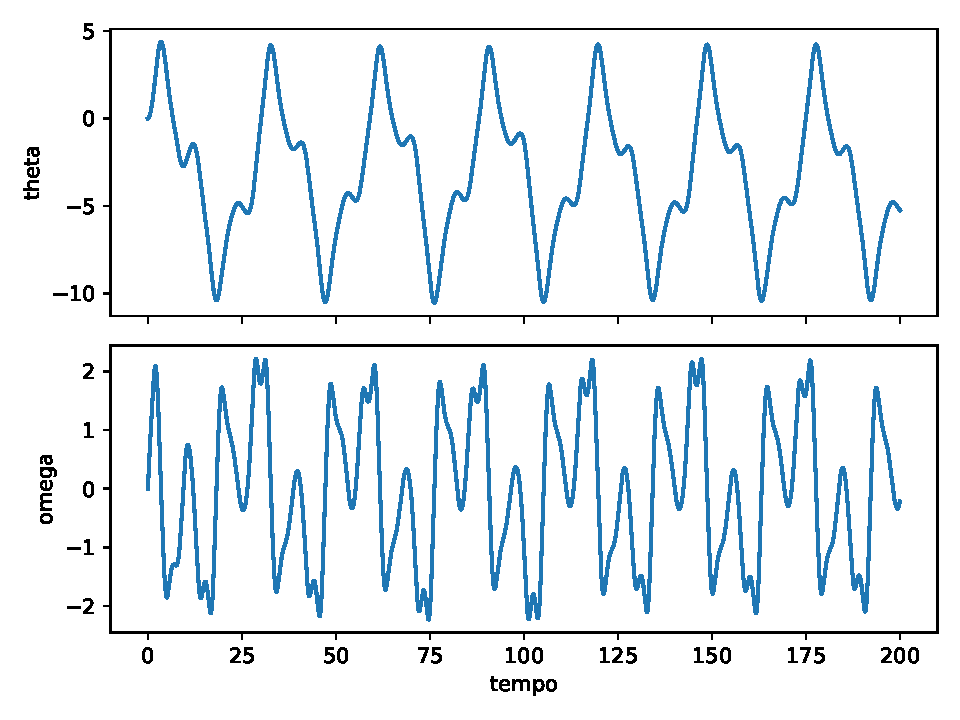
\includegraphics[width=0.7\linewidth]{figs/pendulo}
\end{figure}

\subsection{Método de Euler}
Equações diferenciais ordinárias podem ser resolvidas analiticamente (não abordado neste curso) ou numericamente. Dentre os vários métodos existentes para a solução numérica, a adotada aqui é o método de Euler. Considere a equação $\frac{dx}{dt}=f(x,t)$, com $f(x,t)$ uma função qualquer de $x$ em relação à $t$. Dado um valor inicial $x0$ (usualmente com $t=0$), é possível simular a equação usando pontos discretos com intervalos $\Delta t$ fixos. Cada valor $x_n$ é dado por $x_n=x(t_n=n\Delta t)$. A partir disso, é possível usar o método de Euler avançado para calcular um valor seguinte a partir do valor anterior, ou seja:
$$
x_{n+1}=x_n+f(x_n,t_n)\Delta t
$$

\begin{figure}[htb!]
	\centering
	\caption{Método de Euler}
	\label{fig:euler}
	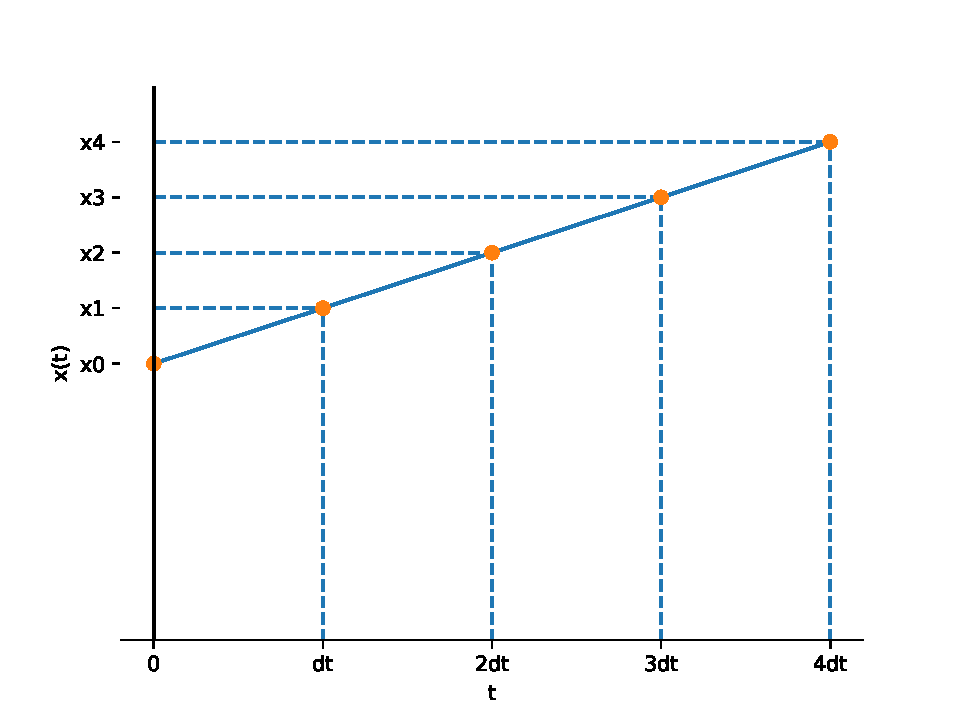
\includegraphics[width=0.7\linewidth]{figs/euler}
\end{figure}

Outros métodos não abordados no curso incluem o método de Euler reverso e o Runge-Kutta de segunda e quarta ordens, que são mais precisos na solução.

\section{Probabilidade}\label{sec:probabilidade}
\begin{itemize}
	\item Experimento aleatório: pode fornecer resultados diferentes a cada vez que se repete da mesma maneira
	\item Espaço amostral (S): conjunto de resultados possíveis para um experimento aleatório (pode ser contínuo ou discreto)
	\item Espaço amostral discreto: conjunto finito ou infinito contável de resultados
	\item Espaço amostral contínuo: intervalo (finito ou infinito) de números reais
	\item Evento (E): subconjunto do espaço amostral
\end{itemize}


\subsection{Probabilidade}
\begin{itemize}
	\item Probabilidade: quantifica a chance de ocorrer o resultado de um experimento aleatório (“A chance de chover hoje é de 30\%")
	\item Axiomas:
	\begin{enumerate}
		\item $P(S)=1$
		\item $0\leq P(E)\leq 1$
		\item $E_1\cap E_2=\emptyset\to P(E_1)+P(E_2)$
	\end{enumerate}
	\item Probabilidade da união: $P(A\cup B)=P(A)+P(B)-P(A\cap B)$
	\item Probabilidade condicional: $P(B|A)=P(A\cap B)/P(A),\quad P(A)>0$
	\item Teorema de Bayes:  $P(A|B)=\frac{P(B|A)P(A)}{P(B)},\quad P(B)>0$\\ % ex. do teste de droga
	\begin{description}
		\item[Exemplo:] Pelo fato de um novo procedimento médico ter se mostrado efetivo na detecção prévia de uma doença, propôs-se um rastreamento médico da população. A probabilidade de o teste identificar corretamente alguém com a doença, dando positivo, é $0,99$, e a probabilidade de o teste identificar corretamente alguém sem a doença, dando negativo, é $0,95$. A incidência da doença na população em geral é $0,0001$. Você fez o teste e o resultado foi positivo. Qual é a probabilidade de você ter a doença?
		\item[Solução:] Seja $D$ o evento em que você tem a doença e seja $S$ o evento é que o teste é positivo. A probabilidade requerida pode ser denotada como $P(D|S)$. A probabilidade de o teste identificar corretamente alguém sem a doença, dando negativo, é $0,95$. Consequentemente a probabilidade de um teste positivo sem a doença é
		$$P(S|D') = 0,05$$
		Do Teorema de Bayes,
		\begin{align*}
			P(D|S)&=P(S|D)P(D)/[P(S|D)P(D)+P(S|D')P(D')]\\
			&=0,99*0,0001/[0,99*0,0001+0,05*(1-0,0001)]\\
			&=1/506=0,002
		\end{align*}
		\item[Interpretação Prática:] A probabilidade de você ter a doença da de um resultado positivo do teste é somente 0,002. Surpreendentemente, embora o teste seja efetivo, no sentido de que $P(S|D)$ é alto e $P(S|D')$ é baixo, por causa da incidência da doença na população em geral ser baixa, as chances são bem pequenas de você realmente ter a doença, mesmo se o teste for positivo
	\end{description}
\end{itemize}


\subsection{Variáveis aleatórias}
\begin{itemize}
	\item Variável aleatória ($X$): função que atribui um número real ($x$) a cada resultado no espaço amostral de um evento aleatório
	\item Discretas: número de pessoas adultas em um ambiente; numero de carros em uma rodovia
	\item Contínuas: corrente elétrica; temperatura; tempo
	\item Função densidade de probabilidade discretas:
	\begin{enumerate}
		\item $f(x_i) \geq 0$ (para todo $x$)
		\item $\sum_{i=1}^n f(x_i)=1$
		\item $f(x_i)=P(X=x_i)$
	\end{enumerate}
	\item Função de distribuição cumulativa discretas: $F(x)=P(X\leq x)=\sum_{x_i\leq x}f(x_i)$
	\begin{enumerate}
		\item $0\leq F(x)\leq 1$
		\item Se $x\leq y$, então $F(x)\leq F(y)$
	\end{enumerate}
	\item Função densidade de probabilidade contínuas:
	\begin{enumerate}
		\item $f(x) \geq 0$ (para todo $x$)
		\item $\int_{-\infty}^\infty f(x)\mathrm{d}x=1$
		\item $P(a\leq X\leq b)=\int_a^b f(x)\mathrm{d}x=$ área sob $f(x)$ de $a$ a $b$ para qualquer $a$ e $b$
	\end{enumerate}
	\item Função de distribuição cumulativa contínuas: $F(x)=P(X\leq x)=\int_{-\infty}^{x}f(u)\mathrm{d}u$
\end{itemize}
\subsubsection{Média e variância}
\begin{itemize}
	\item Média (valor esperado) de uma variável aleatória discreta: $\mu=E(X)=\sum_{x}xf(x)$
	\item Variância de uma variável aleatória discreta: $\sigma^2=V(X)=E(X-\mu)^2$ (desvio-padrão: $\sigma=\sqrt{\sigma^2}$)
	\item Média (valor esperado) de uma variável aleatória contínua: $\mu=E(X)=\int_{\infty}^{\infty}xf(x)\mathrm{d}x$
	\item Variância de uma variável aleatória contínua: $\sigma^2=V(X)=\int_{-\infty}^{\infty}x^2f(x)\mathrm{d}x-\mu^2$ (desvio-padrão: $\sigma=\sqrt{\sigma^2}$)
\end{itemize}

\subsubsection{Distribuição de Poisson}
$$
f(x)=\frac{e^{-\lambda T}(\lambda T)^x}{x!}, x=0,1,2,\dots
$$
\begin{itemize}
	\item $T$: intervalo do evento
	\item $\lambda$: número médio de eventos por intervalo ($0\leq\lambda$)
	\begin{description}
		\item[Exemplo:] Falhas ocorrem ao acaso ao longo do comprimento de um fio delgado de cobre. Suponha que o número de falhas siga a distribuição de Poisson, com uma média de 2,3 falhas por milímetro. Determine a probabilidade de existirem exatamente duas falhas em 1 milímetro de fio.
		\item[Solução:] Seja $X$ o número de falhas em 1 milímetro de fio. Então, $E(X)=2,3$ falhas e
		$$P(X=2) = \frac{e^{-2,3}(2,3)^2}{2!}=0,265$$
		Para determinar a probabilidade de 10 falhas em 5 milímetros de fio, consideramos $X$ o número de falhas em 5 milímetros de fio. Então, $X$ tem uma distribuição de Poisson com
		$$\lambda T=5\text{ mm X }2,3\text{ falhas/mm}=11,5\text{ falhas}$$
		Consequentemente,
		$$P(X=10)=e^{-11,5}\frac{(11,5)^{10}}{10!}=0,113$$
		\item[Interpretação Prática:] Dadas as suposições para um processo de Poisson e um valor para $\lambda$, as probabilidades podem ser calculadas para intervalos arbitrários de comprimento.
	\end{description}
\end{itemize}

\subsubsection{Distribuição normal (Gaussiana)}
$$
f(x)=\frac{1}{\sqrt{2\pi\sigma}}e^{\frac{-(x-\mu)^2}{2\sigma^2}}\qquad-\infty<x<\infty
$$

$$
E(X)=\mu\qquad V(X)=\sigma^2
$$

\begin{figure}[htb!]
	\centering
	\caption{Funções densidade de probabilidade normal para diferentes valores de $\mu$ e $\sigma^2$}
	\label{fig:normal}
	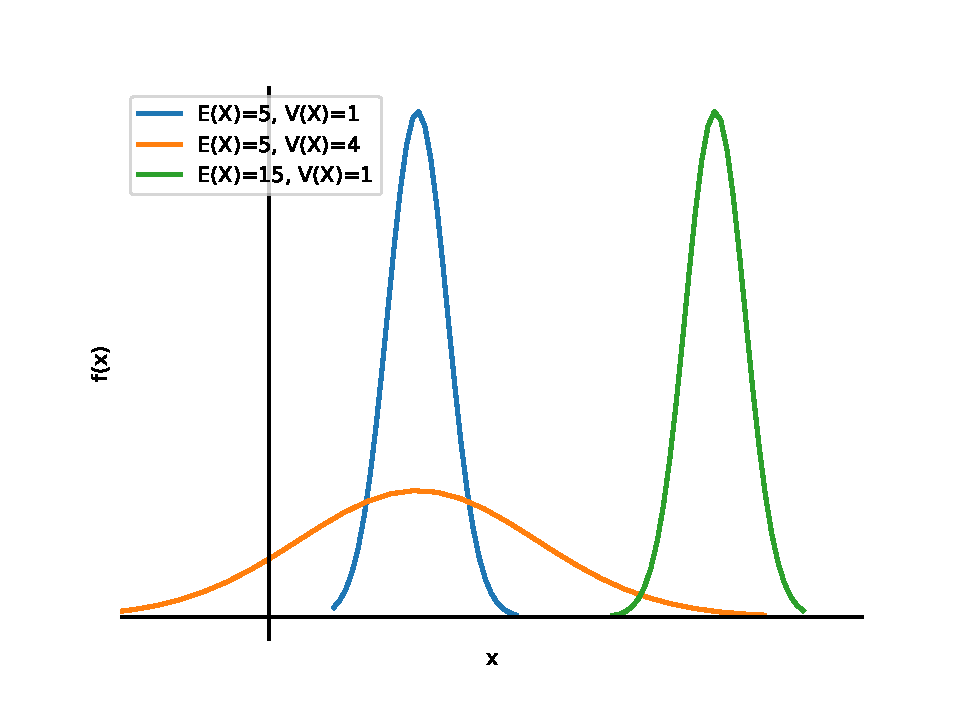
\includegraphics[width=0.7\linewidth]{figs/normal}
\end{figure}


\begin{itemize}
	\item Normal padrão: $\Phi(z)=P(Z\leq z)$, quando $\mu=0$ e $\sigma=1$
\end{itemize}


\section{Noções de algoritmos e programação}\label{sec:algoritmo}
\begin{itemize}
	\item \textbf{Algoritmo}: sequência de instruções para executar uma determinada tarefa. Ex.: algoritmo para lavar as mãos
	\begin{enumerate}
		\centering
		\item Início
		\item Abrir a torneira
		\item Molhar as mãos
		\item Ensaboar as mãos
		\item Molhar as mãos
		\item Secar as mãos
		\item Fim
	\end{enumerate}
	
	\item \textbf{Programa}: conjunto de instruções escritas em um arquivo com regras específicas
	\begin{verbatim}
		print("Olá, mundo!")
	\end{verbatim}
	\item \textbf{Linguagem de programação}: converte o programa escrito em ações no computador (ex.: \textit{Python}, \textit{C++}, \textit{Java})
\end{itemize}

\begin{figure}[htb!]
	\centering
	\caption{Do código para e/s}
	\label{fig:codigoio}
	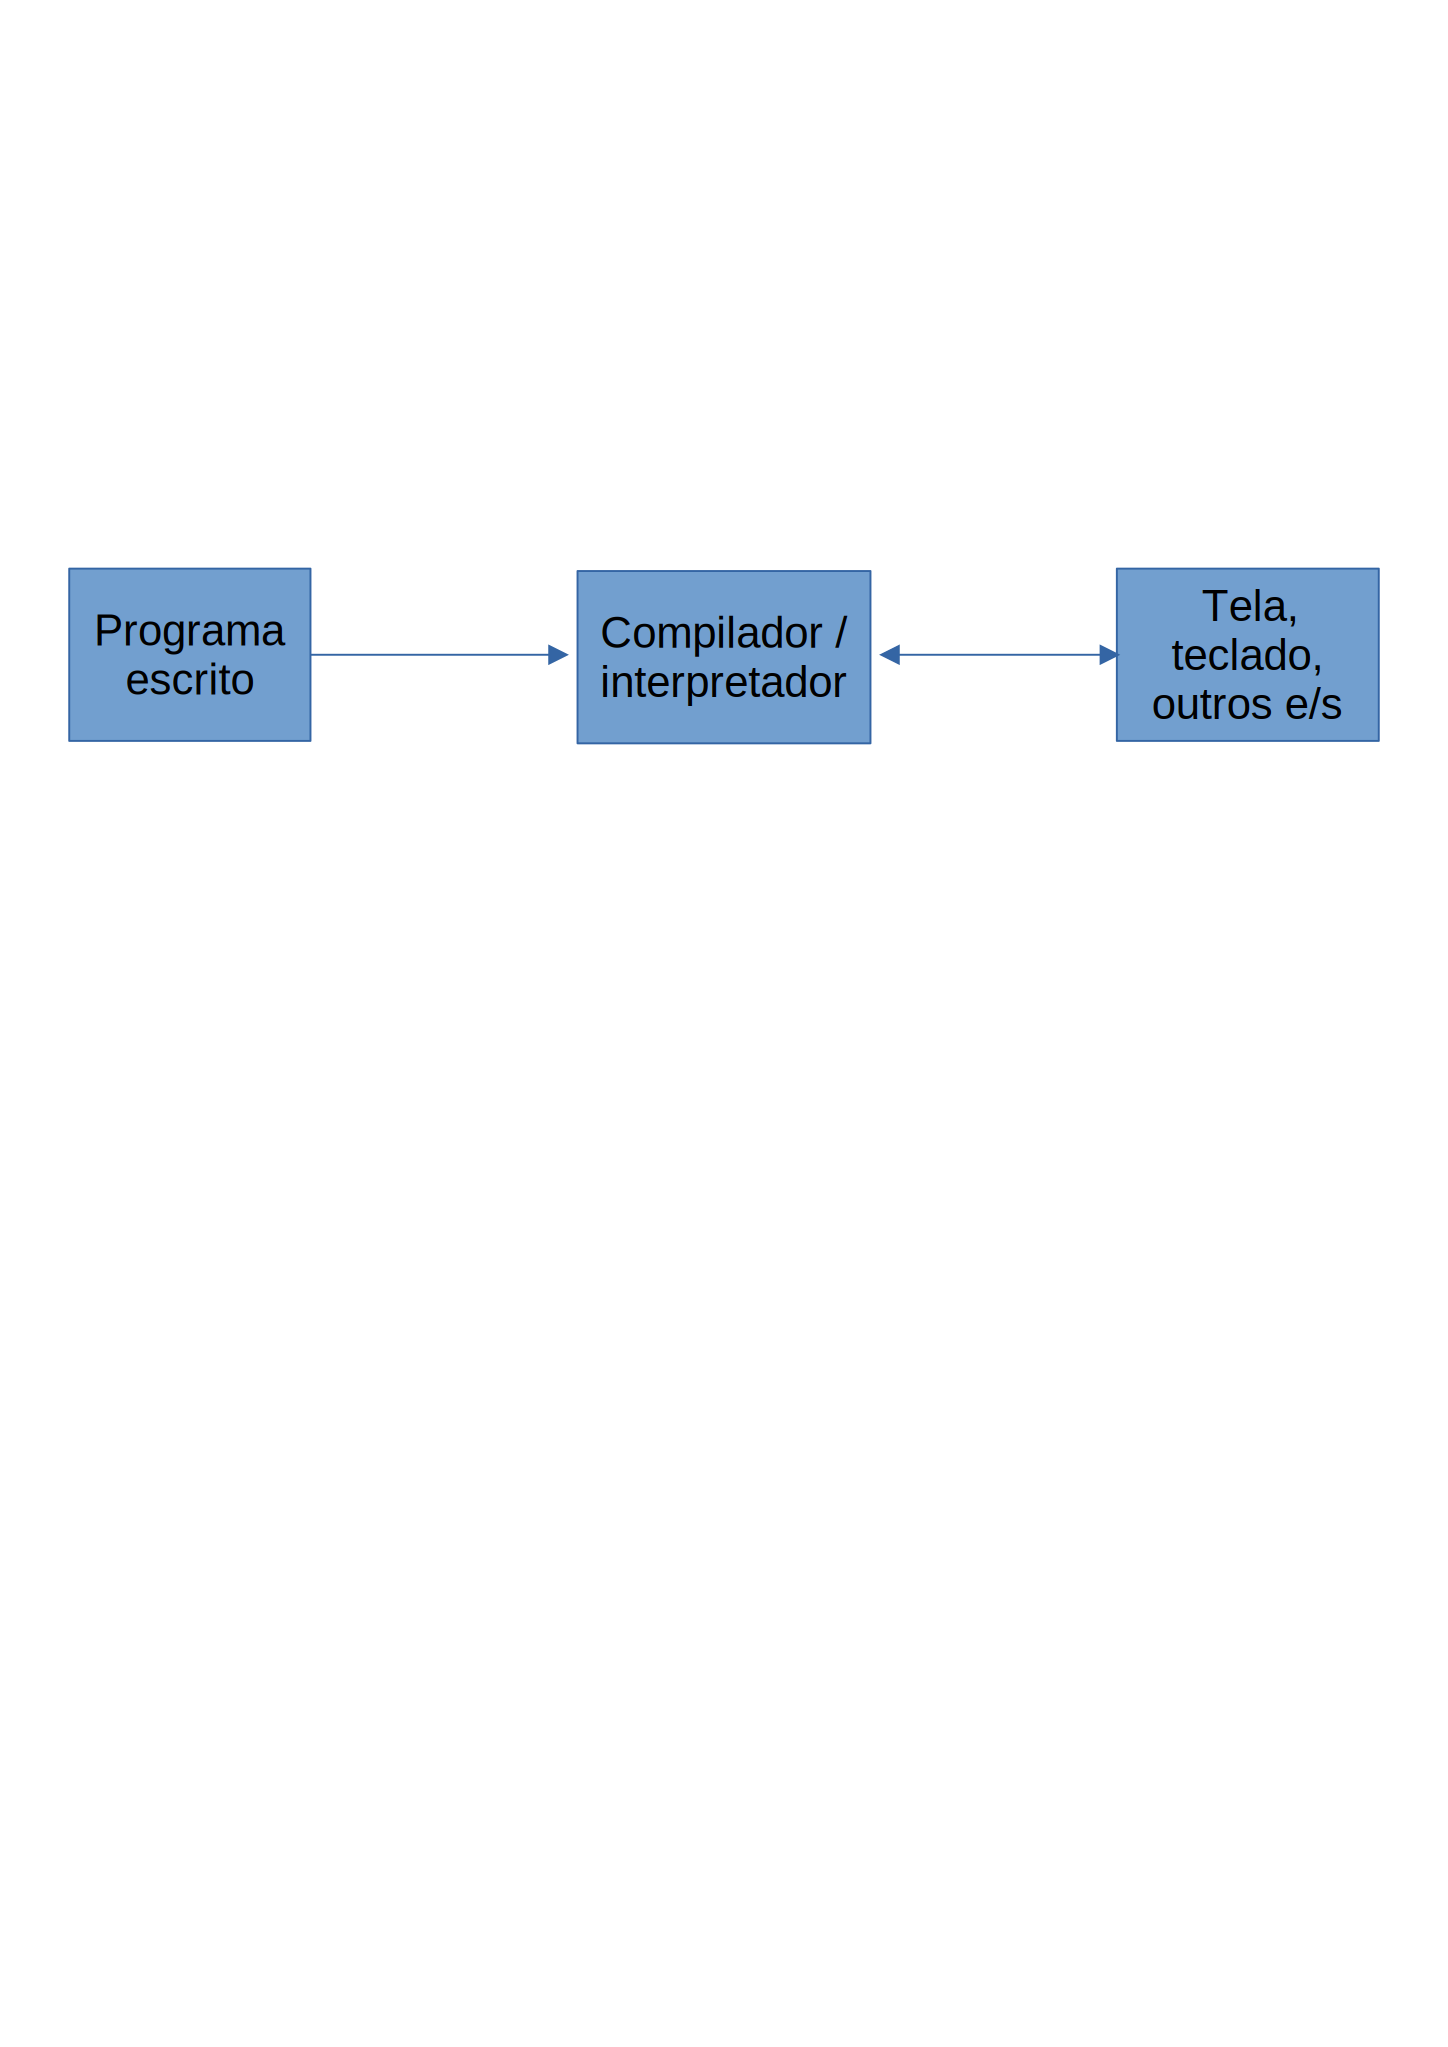
\includegraphics[width=0.7\linewidth]{figs/codigo_io}
\end{figure}

\SetKwComment{Comment}{/* }{ */}
\begin{algorithm}
	\caption{Exemplo}\label{alg:ohm}
	\KwData{$n \geq 0$}
	\KwResult{$y = x^n$}
	$y \gets 1$\;
	$X \gets x$\;
	$N \gets n$\;
	\While{$N \neq 0$}{
		\eIf{$N$ é par}{
			$X \gets X \times X$\;
			$N \gets \frac{N}{2}$ \Comment*[r]{Este é um comentário}
		}{\If{$N$ é impar}{
				$y \gets y \times X$\;
				$N \gets N - 1$\;
			}
		}
	}
\end{algorithm}

\chapter{Temas apresentados}\label{cap:temas}
\section{Introdução}\label{sec:temas_intro}

\section{Modelos de neurônio}\label{sec:modelos}

\section{Conexões entre neurônios}\label{sec:conexoes}

\section{Plasticidade de curta duração}\label{sec:plasticidade}

\section{Simuladores neuronais}\label{sec:simuladores}

\section{Redes neuromórficas}\label{sec:redes}

% ----------------------------------------------------------
% Considerações Finais
% ----------------------------------------------------------
\chapter{Considerações finais}\label{cap:conclusoes}
Este trabalho apresentou uma série de conteúdos para a execução de um curso introdutório de neurociência computacional, voltado para diversos públicos, servindo como um guia de execução. Baseado em algumas execuções do curso, uma possível sequência didática para o mesmo é mostrada na Tabela~\ref{tab:sequencia_didatica}.
\begin{table}[tb]
	\IBGEtab{
		\caption{Proposta de sequência didática}
		\label{tab:sequencia_didatica}
	}{
	\begin{tabular}{|c|c|p{8cm}|}
	\hline
	Número da aula & Tema & Conteúdo \\
	\hline
	1 & Apresentação da disciplina & Apresentação do estado da arte \\
	\hline
	2-4 & Introdução & Neurobiologia; equações diferenciais; introdução ao Python \\
	\hline
	5-9 & Modelos de neurônio de disparo & Modelos LIF, ELIF, AELIF, Izhikevich, Hodgkin-Huxley \\
	\hline
	10-17 & Conexões entre neurônios & Sinapses; Sinapses dinâmicas; Multi-estabilidade; Modelos de Wilson-Cowan; Aprendizado \\
	\hline
	18-21 & Inteligência artificial & Redes neurai; Redes neuromórficas \\
	\hline
	22-24 & Conclusão & Apresentações/entregas de trabalhos; Avaliação da disciplina \\
	\hline
	\end{tabular}
}{
\fonte{o autor (\the\year)}
}
\end{table}
Também baseado em execuções do curso, foi elaborada a proposta de atividades avaliativas, referentes a cada capítulo apresentado, como segue:
\begin{alineas}
	\item Introdução: questões simples de neurobiologia, equações diferenciais e implementações de códigos em Python;
	\item modelos: alterações de parâmetros nos modelos LIF, ELIF e/ou AELIF;
	\item conexões: implementação de circuitos de multi-estabilidade com o modelo de Wilson-Cowan;
	\item tarefa final: implementação de codificação para a rede de disparo.
\end{alineas}

A proposta de execução do curso é utilizando o Google Colaboratory (Colab), que fornece um ambiente de programação em Python gratuito, incluindo recursos de \textit{hardware} robustos para aplicações de aprendizado de máquina.
%TODO: citação bisong google colaboratory
Como exibido na Figura~\ref{fig:colab}, o Colab é executado a partir de um \textit{Notebook}, que facilita a execução e reprodução de códigos e conteúdos em conjunto.
%TODO: citação interactive
Todos os códigos-fonte utilizados durante o curso, incluindo os que geram algumas das imagens deste texto, estão disponíveis em repositório online\footnote{\url{https://gitlab.com/weversonvn/intro_neurocomp}}, de maneira gratuita e com uma licença permissiva livre para uso.
\begin{figure}[tb]
	\centering
	\caption[Ambiente do Google Colaboratory com o conteúdo de neurônios de disparo]{Ambiente do Google Colaboratory com o conteúdo de neurônios de disparo}
	\label{fig:colab}
	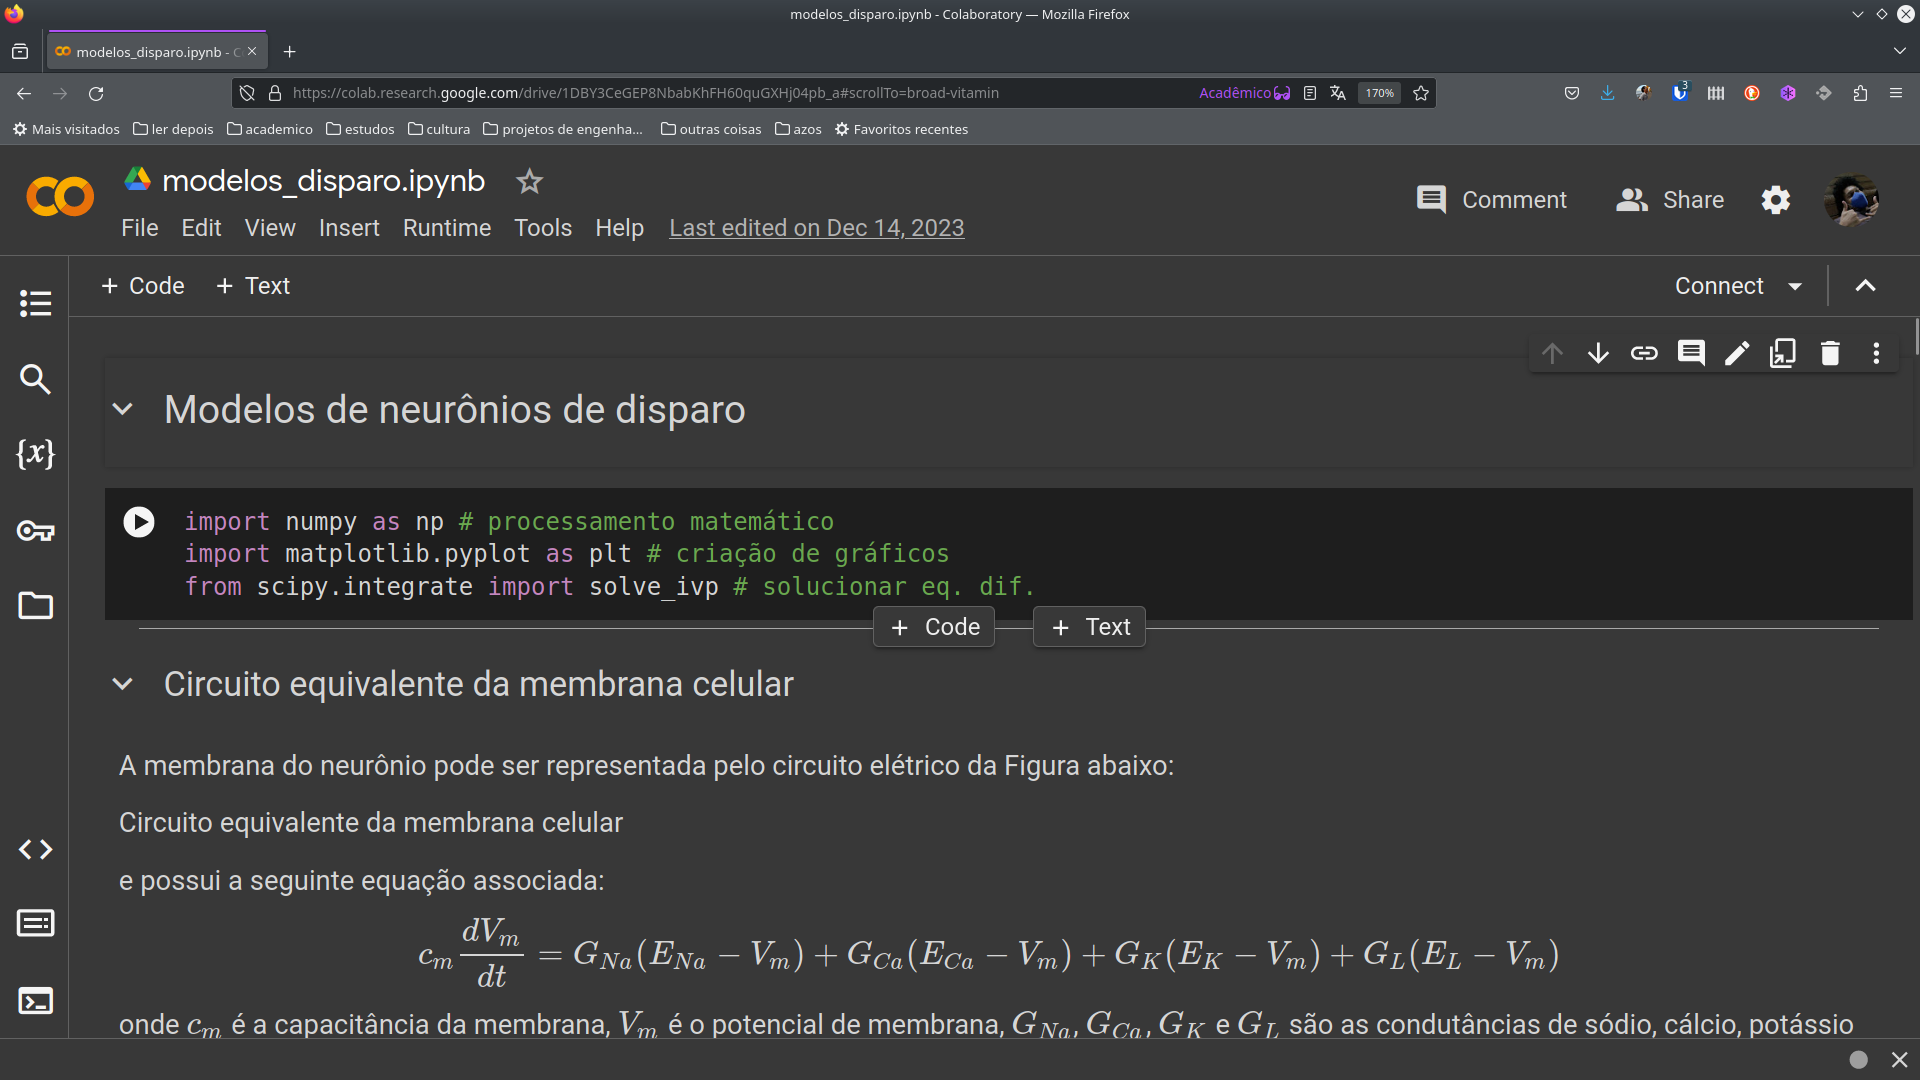
\includegraphics[width=0.7\linewidth]{figs/colab}
	\legend{Fonte: o autor (\the\year)}
\end{figure}

Possíveis melhorias para o curso começam pelo refinamento dos conteúdos já existentes, baseado nas considerações que venham a ser obtidas por eventuais alunos que o façam, como a alteração da ordem dos conteúdos, maior detalhamento de algum tópico específico, diminuição de outros. Além disso, um material voltado para exercícios pode ser bastante útil, tanto dos conteúdos teóricos quanto dos práticos, com destaque para tarefas em Python voltadas para cursos onde o público alvo não tem grande familiaridade com a linguagem ou com programação.

Como conteúdos novos pode-se incluir a simulação de modelos multi-compartimento, com destaque para a estimulação elétrica axonal, para estudar a propagação do potencial de ação ao longo do axônio.
%TODO: citação rattay a model
Outra possibilidade é a análise de sinais de eletroencefalograma (EEG), que são respostas elétricas obtidas das atividades cerebrais, podendo ser utilizadas para associações com comorbidades, como depressão e ansiedade.
%TODO: cavanagh multiple
Por fim, a apresentação de pacotes do Python voltados para análises semelhantes às apresentadas no curso pode ser incluído, uma vez que o uso destes potencialmente se torna mais simplificado com o entendimento obtido a partir do conteúdo deste trabalho.

% ---

% ----------------------------------------------------------
% ELEMENTOS PÓS-TEXTUAIS
% ----------------------------------------------------------
\postextual
% ----------------------------------------------------------

% ----------------------------------------------------------
% Referências bibliográficas (obrigatório - NBR 6023)
% ----------------------------------------------------------
% Os elementos essenciais são: autor(es), título, edição, local, editora e data de publicação
%  Quando se tratar de obras consultadas online,  também  são  essenciais  as  informações  sobre  o  endereço  eletrônico, apresentado  entre  os  sinais  <  >,  precedido  da  expressão  Disponível  em:  e  a  data  de  acesso  ao  documento,  precedida  da expressão Acesso em:, opcionalmente acrescida dos dados referentes a hora, minutos e segundos

% o template já faz no formato adequado
% eu fiz um arquivo .bib separado que é importado aqui
\bibliography{neurocomp}
% ---

% antes do apêndices um item opcional é o glossário
% se incluído é em ordem alfabética

% ----------------------------------------------------------
% Apêndices (opcional)
% ----------------------------------------------------------

% ---
% Inicia os apêndices
% ---
%\begin{apendicesenv}
	
	% Imprime uma página indicando o início dos apêndices
	% a norma não diz para criar essa página
%	\partapendices

% usar um include com \chapter para cada apêndice
	
%\end{apendicesenv}
% ---

% ----------------------------------------------------------
% Anexos (opcional)
% ----------------------------------------------------------

% ---
% Inicia os anexos
% ---
%\begin{anexosenv}
	
	% Imprime uma página indicando o início dos anexos
	% novamente a norma não diz para criar essa página
%	\partanexos

% novamente usar um include com \chapter para cada anexo
% ou usar \includepdf caso seja documento externo (o mais provável no caso de anexo)
	
%\end{anexosenv}

% o último item opcional é o índice
% se incluído é conforme a NBR 6034

\end{document}
